\chapter{Example Chapter}\label{ch:ExampleChapter}
  This chapter aims to provide examples how how to structure and create specific components in your thesis document. 
  The very first one is showing a citation, like the one at the end of this sentence \cite{TEST}. 
  The second shows how to create more than one citation and how they are grouped \cite{testone,cite2,cite3,cite4,cite5}.
  This sentence shows how a gap in the citations is handled \cite{testone,cite2,cite3,cite5}. 
  \section{Tables}
	
  % X - Justified (Equal Spacing)
  % L - Left Aligned (Equal Spacing)
  % C - Center Aligned (Equal Spacing)
  % R - Right Aligned (Equal Spacing)
  % l - Left Aligned (Fit to Contents)
  % c - Center Aligned (Fit to Contents)
  % r - Right Aligned (Fit to Contents)
  
  \begin{table}[!htb]
    \caption{This is a basic table}
    \centering
    \begin{tabularx}{0.75\textwidth}{LCR} 
      % Equally spaced cells that are left, center, and right aligned. 
      % The entire table will be 75% the width of the text.
      \hline
      \textbf{Left Aligned Title} & \textbf{Centered Title} & \textbf{Right Aligned Title} \\\hline
      This is left aligned & This is centered & This is right aligned \\
      This is left aligned & This is centered & This is right aligned \\
      This is left aligned & This is centered & This is right aligned \\
      This is left aligned & This is centered & This is right aligned \\\hline
    \end{tabularx}
    \label{tab:basicTable}
  \end{table}
  
  \begin{table}[!htb]
    \caption{This is a complex table.}
    \centering
    \begin{tabularx}{\textwidth}{lCR}
      % Left most cell is fitted to the content.
      % The center and right columns are equally spaced cells that are center, and right aligned. 
      % The entire table will be 75% the width of the text.
      \hline
      \multirow{2}{*}{\textbf{This is two row\quad}} & \multicolumn{2}{c}{\textbf{This is two columns}}\\\cline{2-3} % \cline draws a partial line across cells #-#
       & \textbf{Centered Title} & \textbf{Right Aligned Title} \\\hline
      \multirow{2}{*}{This is two row} & This is centered & This is right aligned \\
       & This is centered & This is right aligned \\\cline{1-1}
      \multirow{2}{*}{This is two row} & This is centered & This is right aligned \\
       & This is centered & This is right aligned \\\hline
    \end{tabularx}
    \label{tab:complexTable}
  \end{table}
  
  
  \section{Figures}
  This section will provide examples of how to create figures, and different types of multi/sub-figures. 
  Additionally, if you have many figures in a section and they are bleeding too much into the following sections a \texttt{\textbackslash{}clearpage} command can be issued before the next section. 
  However, note that this will force the next section to begin on a new page. 
  Note that the first ``figure'' is actually a plate; a plate is the proper title associated with a \textit{photograph}, using the environment `plate' instead of `figure' and command \texttt{\textbackslash{listofplates}} will generate everything for you.
  \begin{plate}[!htb]
    \centering
    \includegraphics[width=0.7\textwidth]{example-image}
    \caption{This is an example of a single image plate.}
    \label{fig:singleImage}
  \end{plate}
  
  \begin{figure}[!htb]
    \centering
    \begin{subfigure}{0.45\textwidth}
      \includegraphics[width=\textwidth]{example-image}
      \caption{} % Leave blank for just letter
      \label{fig:doubleImage:a}
    \end{subfigure}
    ~
    \begin{subfigure}{0.45\textwidth}
      \includegraphics[width=\textwidth]{example-image}
      \caption{} % Leave blank for just letter
      \label{fig:doubleImage:b}
    \end{subfigure}
    \caption{This is an example of a double image figure.}
    \label{fig:doubleImage}
  \end{figure}
  
  \begin{figure}[!htb]
    \centering
    \hspace*{\fill}% Adds space to left of top image (prevents two images from going to top)
    \begin{subfigure}{0.45\textwidth}
      \includegraphics[width=\textwidth]{example-image}
      \caption{} % Leave blank for just letter
      \label{fig:tripleImage1:a}
    \end{subfigure}
    \hspace*{\fill} % Adds space to right of top image (prevents two images from going to top)
    \par\vspace{1em}% Adds space between upper and lower images
    \begin{subfigure}{0.45\textwidth}
      \includegraphics[width=\textwidth]{example-image}
      \caption{} % Leave blank for just letter
      \label{fig:tripleImage1:b}
    \end{subfigure}
    ~ % Adds space between the two lower figures
    \begin{subfigure}{0.45\textwidth}
      \includegraphics[width=\textwidth]{example-image}
      \caption{} % Leave blank for just letter
      \label{fig:tripleImage1:c}
    \end{subfigure}
    \caption{This is an example of a triple image figure.}
    \label{fig:tripleImage1}
  \end{figure}
  
  \begin{figure}[!htb]
    \centering
    \hspace*{\fill}% Adds space to left of top image (prevents two images from going to top)
    \begin{subfigure}{0.90\textwidth+1em} % 0.9 = 0.45 + 0.45, and 1em is the width of ~
      \includegraphics[width=\textwidth]{example-image}
      \caption{} % Leave blank for just letter
      \label{fig:tripleImage2:a}
    \end{subfigure}
    \hspace*{\fill} % Adds space to right of top image (prevents two images from going to top)
    \par\vspace{1em}% Adds space between upper and lower images
    \begin{subfigure}{0.45\textwidth}
      \includegraphics[width=\textwidth]{example-image}
      \caption{} % Leave blank for just letter
      \label{fig:tripleImage2:b}
    \end{subfigure}
    ~ % Adds space between the two lower figures
    \begin{subfigure}{0.45\textwidth}
      \includegraphics[width=\textwidth]{example-image}
      \caption{} % Leave blank for just letter
      \label{fig:tripleImage2:c}
    \end{subfigure}
    \caption{This is a second example of a triple image figure.}
    \label{fig:tripleImage2}
  \end{figure}
  
  \begin{figure}[!htb]
    \centering
    \begin{subfigure}{0.45\textwidth}
      \includegraphics[width=\textwidth]{example-image}
      \caption{} % Leave blank for just letter
      \label{fig:quadImage:a}
    \end{subfigure}
    ~ % Adds space between the two top figures
    \begin{subfigure}{0.45\textwidth}
      \includegraphics[width=\textwidth]{example-image}
      \caption{} % Leave blank for just letter
      \label{fig:quadImage:b}
    \end{subfigure}
    \par\vspace{1em} % Adds space between upper and lower images
    \begin{subfigure}{0.45\textwidth}
      \includegraphics[width=\textwidth]{example-image}
      \caption{} % Leave blank for just letter
      \label{fig:quadImage:c}
    \end{subfigure}
    ~ % Adds space between the two lower figures
    \begin{subfigure}{0.45\textwidth}
      \includegraphics[width=\textwidth]{example-image}
      \caption{} % Leave blank for just letter
      \label{fig:quadImage:d}
    \end{subfigure}
    \caption{This is an example of a quad image figure.}
    \label{fig:quadImage}
  \end{figure}
  
  \clearpage % forces the remaining images (floats to be placed)
  \section{Graphs \& Plots}
  In the following section there will be a few examples of how to generate plots.
  For more information on how to create plots, \href{https://mirror.its.dal.ca/ctan/graphics/pgf/contrib/pgfplots/doc/pgfplots.pdf}{\textcolor{blue}{\underline{here}}} is the manual for pgfplots.
  \begin{figure}[htb!]
    \centering
    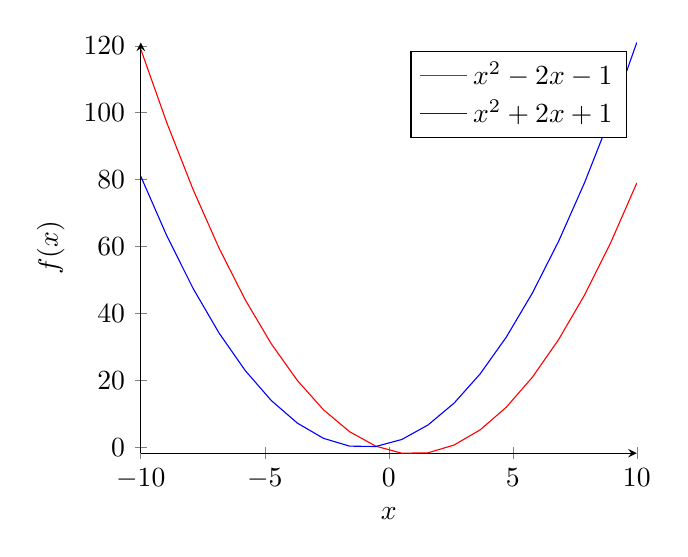
\begin{tikzpicture}
      \begin{axis}[
          width=0.65\textwidth,
          axis lines = left,
          xlabel = \(x\),
          ylabel = {\(f(x)\)},
      ]
        %Below the red parabola is defined
        \addplot [
            domain=-10:10, 
            samples=20, 
            color=red,
        ]
        {x^2 - 2*x - 1};
        \addlegendentry{\(x^2 - 2x - 1\)}
        %Here the blue parabola is defined
        \addplot [
            domain=-10:10, 
            samples=20, 
            color=blue,
            ]
            {x^2 + 2*x + 1};
        \addlegendentry{\(x^2 + 2x + 1\)}
      \end{axis}
    \end{tikzpicture}
    \caption{Plot of two parabola.}\label{fig:parabolaplot}
  \end{figure}
  
  \begin{figure}[htb!]
    \centering
    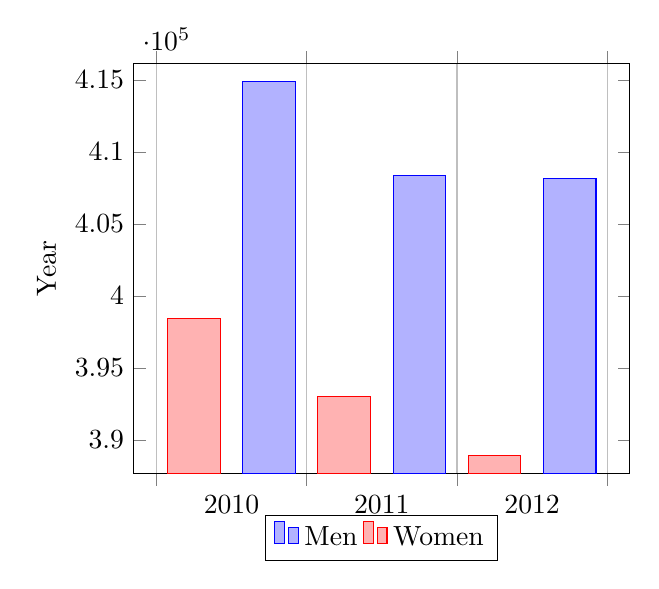
\begin{tikzpicture}
      \begin{axis}[
        width=0.65\textwidth,
        x tick label style={
          /pgf/number format/1000 sep=},
        ylabel=Year,
        enlargelimits=0.05,
        legend style={at={(0.5,-0.1)},
        anchor=north,legend columns=-1},
        ybar interval=0.7,
      ]
      \addplot 
        coordinates {(2012,408184) (2011,408348)
           (2010,414870) (2009,412156)};
      \addplot 
        coordinates {(2012,388950) (2011,393007) 
          (2010,398449) (2009,395972)};
      \legend{Men,Women}
      \end{axis}
    \end{tikzpicture}
    \caption{Example of a Bar Graph.}\label{fig:bargraph}
  \end{figure}
  
  \begin{figure}[htb!]
    \centering
    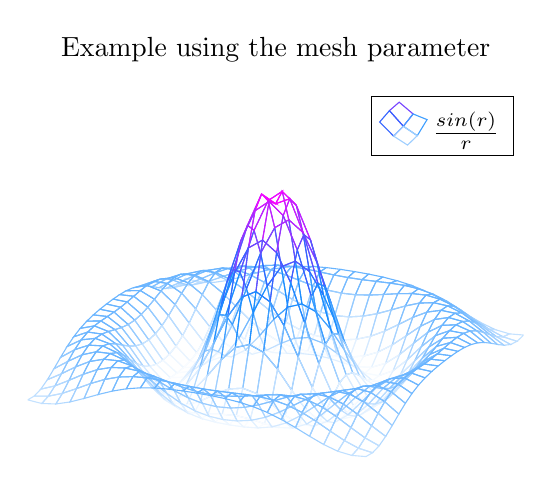
\begin{tikzpicture}
      \begin{axis}[
          width=0.65\textwidth,
          title=Example using the mesh parameter,
          hide axis,
          colormap/cool,
      ]
      \addplot3[
          mesh,
          samples=25,
          domain=-8:8,
      ]
      {sin(deg(sqrt(x^2+y^2)))/sqrt(x^2+y^2)};
      \addlegendentry{\(\frac{sin(r)}{r}\)}
      \end{axis}
    \end{tikzpicture}
    \caption{Example of a 3D Plot}\label{fig:3dplot}
  \end{figure}
  
  \begin{figure}[htb!]
    \centering
    \begin{tikzpicture}
      \begin{axis}[
          width=0.65\textwidth,
          enlargelimits=true,
      ]
      \addplot+[
          only marks,
          scatter,
          mark=*,
          mark size=2.9pt]
      table[meta=ma]
      {./Chapters/scattered_example.dat};
      \end{axis}
      \end{tikzpicture}
    \caption{Example of a Scatter Plot.}\label{fig:scatterplot}
  \end{figure}
  
  \clearpage
  \section{Equations}
  The following equation has no referencing number:
  \nonumeq{E & = m\ c^2}
  
  \Cref{eq:quickEq} has a reference to it though. Or for more control the source for \Cref{eq:quickEq} can be written out fully as it was for \Cref{eq:quickEq2}.
  
  \numeq{pi & = 3.1415...}{eq:quickEq} % shorthand for the following way of writing equations.
  \begin{align}\label{eq:quickEq2}
    e & = 2.7183...
  \end{align}
  
  If you have multiple equations that you want arranged very neatly, use the align environment and you can assign individual equations numbers as shown in \Cref{eq:multiref:a,eq:multiref:b,eq:multiref:c}.
  \begin{align}%Note: Alignment happens at the "=" character
    \label{eq:multiref:a} Equation1 & = 1\\
    \label{eq:multiref:b} Equation2 & = 2 + 2\\
    \label{eq:multiref:c} Equation3 & = 3 + 3 + 3
  \end{align}
  
  
  
  \printreferences % Add a Reference Section to the end of the Chapter.
